%!TEX root = ../ArticleCalib_main.tex


%%%%%%%%%%%%% FIGURE 7 et 8 BBR theorique

\begin{figure}[htbp]
\begin{center}
\captionsetup[subfigure]{position=top, labelfont=bf, textfont=normalfont, singlelinecheck=off, justification=raggedright }

\subfloat[]{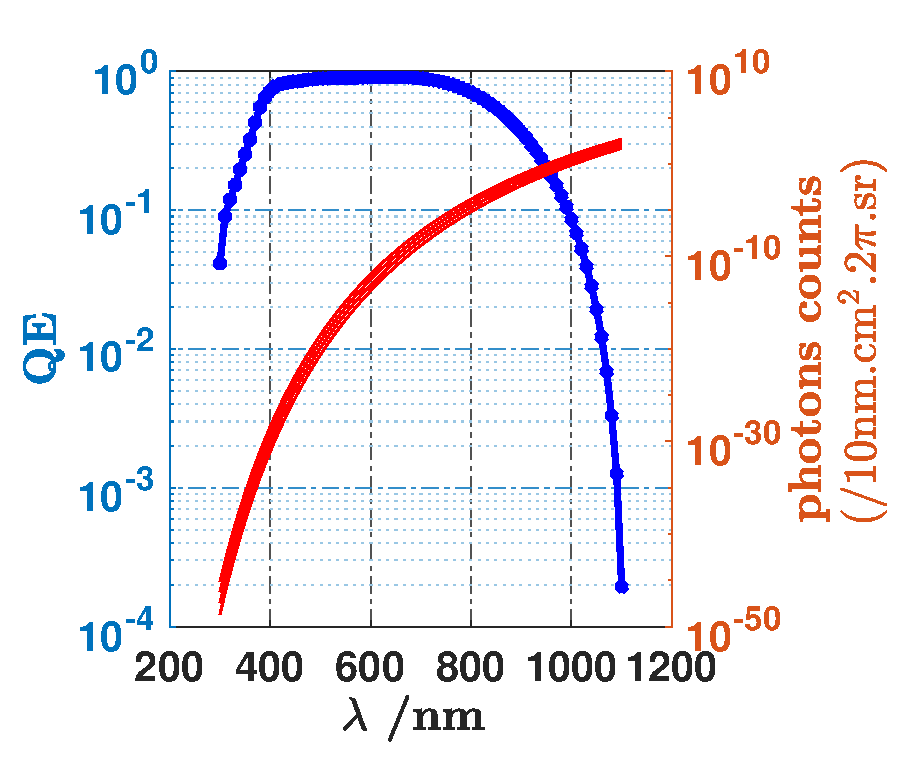
\includegraphics[width=0.4\linewidth]{fig7_8_BBRtheo/fig7A_nuvucamBBR15202530semilogy_QEdoubleax.eps}\label{fig:BBRtheo1:A}} \qquad
\subfloat[]{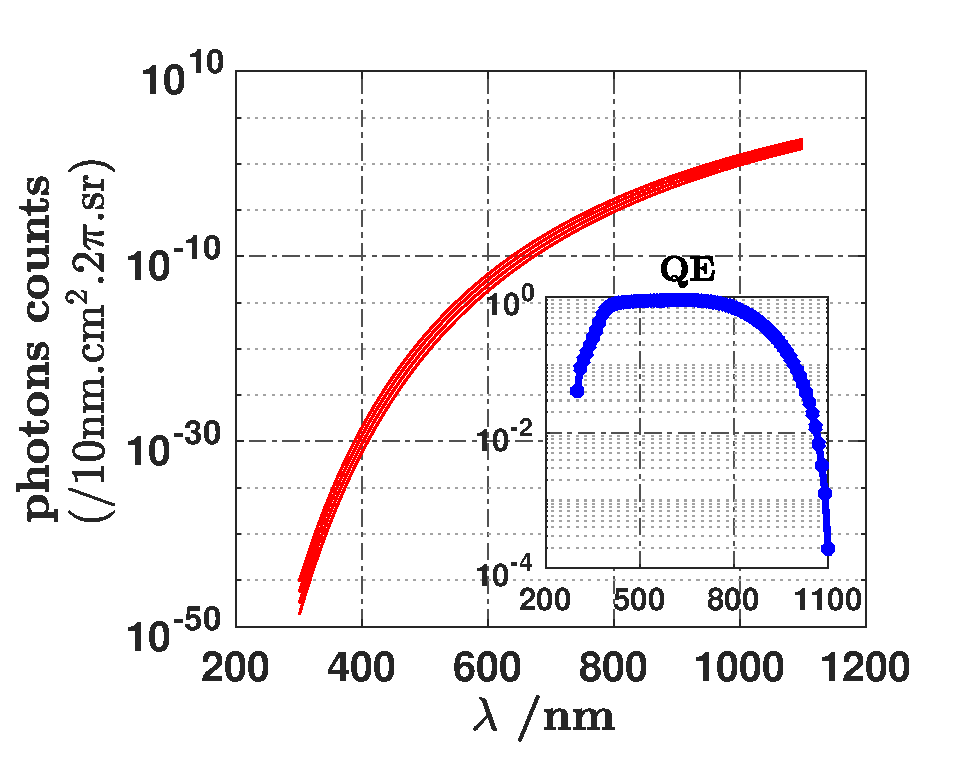
\includegraphics[width=0.4\linewidth]{fig7_8_BBRtheo/fig7A_nuvucamBBR15202530semilogy_QEinsert.eps}\label{fig:BBRtheo1:B}} \\

\subfloat[]{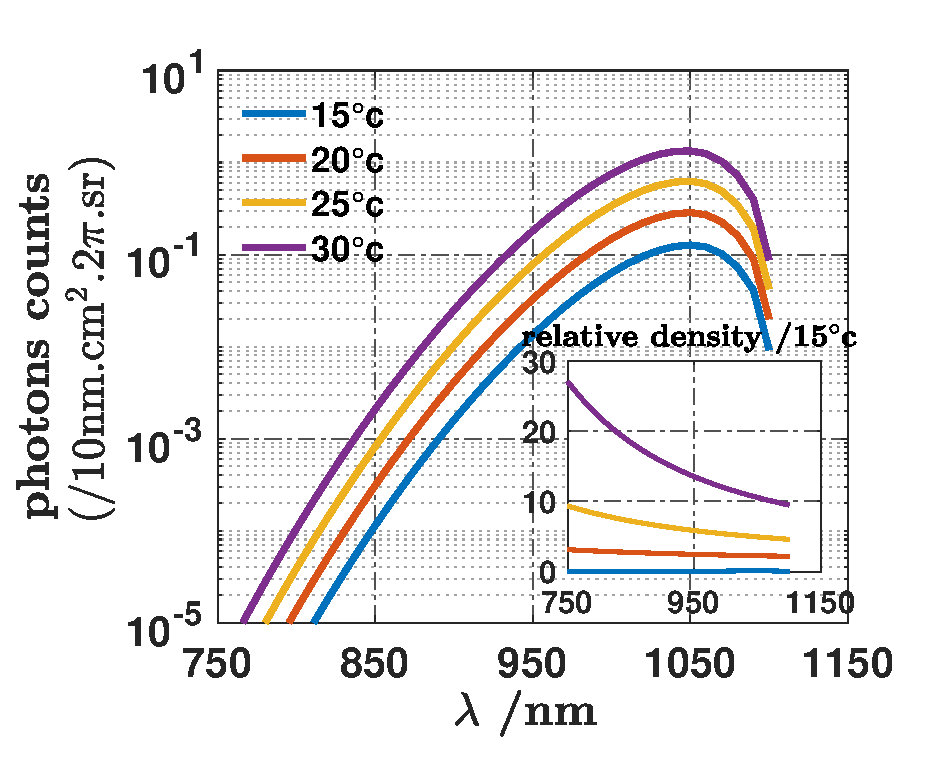
\includegraphics[width=0.4\linewidth]{fig7_8_BBRtheo/fig7B_nuvucamBBR_Tau600sPlanckBGsat_inclreldens15.eps}\label{fig:BBRtheo1:C}} \\

\subfloat[]{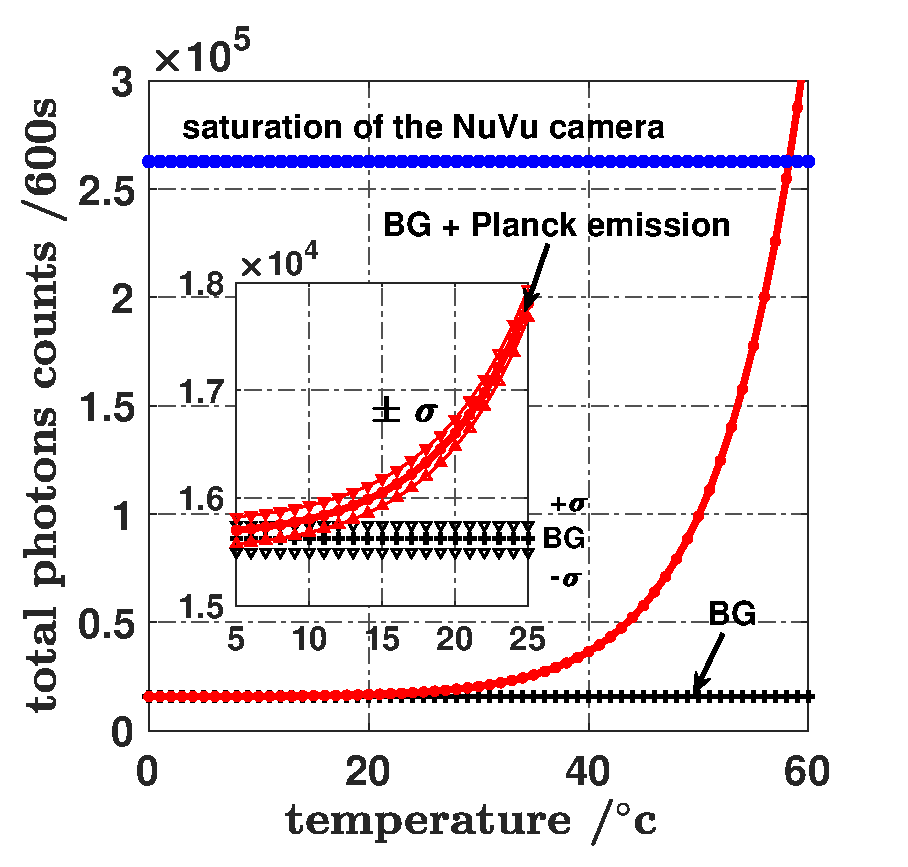
\includegraphics[width=0.5\linewidth]{fig7_8_BBRtheo/fig7C_nuvucamBBR_Tau600sPlanckBGsat_incl.eps}\label{fig:BBRtheo1:D}}

\caption{{\bf Black Body radiation spectra and spectral density of thermal radiation}.  The BBR is presented for increasing temperatures of 15, 20, 25 and 30 celsius degrees integrated over 10nm of wavelength during 1 second for 1 cm$^2$ surface over $2\pi$ sr. The inserted figure shows a zoom over $\lambda = [0.7 - 1.1]$ nm, representing the spectral density relative to 15$^o$c (\subref{fig:BBRtheo1:C}.)
{\bf Quantum Efficiency of the Nuvu Camera and spectral density of thermal radiation}.  Y axe is in logarithmic scale to show the dramatic decrease of the detectability when going toward shorter wavelength, the quantum efficiency of the NüVü camera is represented along with the spectral density of the thermal radiation.  (\subref{fig:BBRtheo1:A} and \subref{fig:BBRtheo1:B}.)
{\bf Model : NuVu Camera counts (N1) as a function of the temperature  }.  The N1 is given by summing the BackGround (BG) noise of the NuVu camera and the detected flux of the BBR. This detected flux is found by integrating the BBR over the QE as a function of $\lambda$ for a $\tau = 600s$. The pixels saturation level is shown ($N1 = \sum_{ij} pixels$). The inclusion shows the temperatures for which the detected Planck flux emission begins to be significantly detectable  (\subref{fig:BBRtheo1:D}.)}
\label{fig:BBRtheo1}
\end{center}
\end{figure}


\begin{figure}[htbp]
\begin{center}
\captionsetup[subfigure]{position=top, labelfont=bf, textfont=normalfont, singlelinecheck=off, justification=raggedright }

\subfloat[]{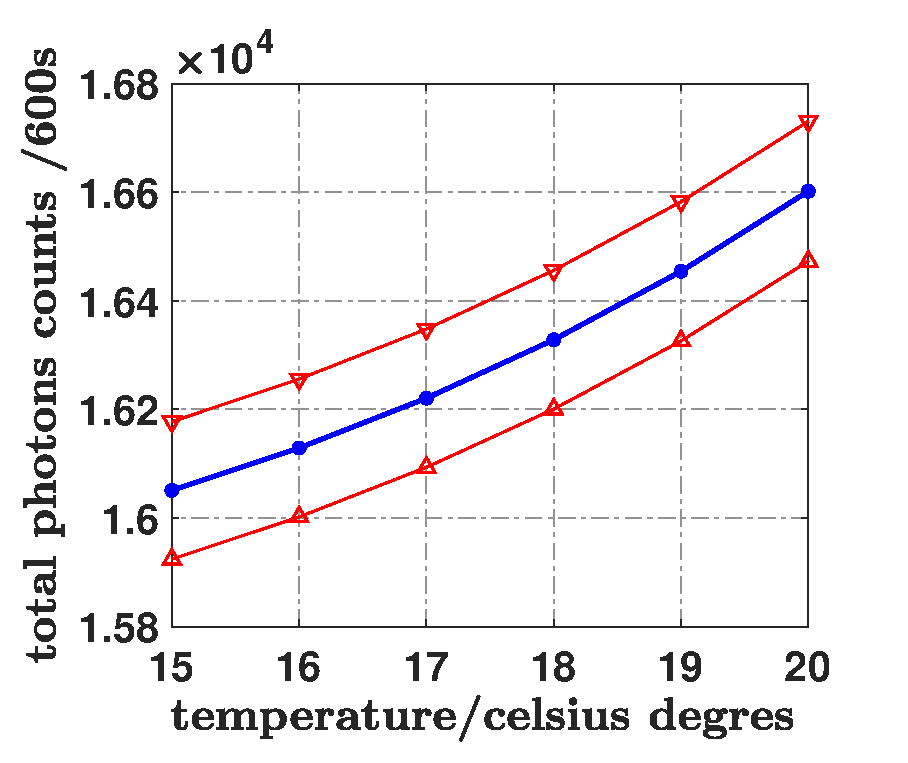
\includegraphics[width=0.4\linewidth]{fig7_8_BBRtheo/fig8A_nuvucamBBR_Tau600sPlanckTemp1520.eps}} \qquad
\subfloat[]{\includegraphics[width=0.4\linewidth]{fig7_8_BBRtheo/fig8B_nuvucamBBR_Tau600sPlanckTemp2025.eps}}\\

\subfloat[]{\includegraphics[width=0.4\linewidth]{fig7_8_BBRtheo/fig8C_nuvucamBBR_Tau600sPlanckTemp2530.eps}}\qquad
\subfloat[]{\includegraphics[width=0.4\linewidth]{fig7_8_BBRtheo/fig8D_nuvucamBBR_Tau600sPlanckTemp3035.eps}}\\

\subfloat[]{\includegraphics[width=0.4\linewidth]{fig7_8_BBRtheo/fig8E_nuvucamBBR_Tau600sPlanckTemp3540.eps}}\qquad

\caption{{\bf NuVu Camera counts (N1) as a function of the temperature : zoom}. Here is shown how the Noise Equivalent Temperature Difference (NETD) decrease dramatically with the increasing of the temperature. Arrows are showing the standard deviation of the measure according to the model. (A), (B), (C), (D), (E)  from [15 to 20], [20 to 25], [25 to 30], [30 to 35], [35 to 40] celsius degrees respectively. }
\label{fig:BBRtheo2}
\end{center}
\end{figure}


